% Options for packages loaded elsewhere
\PassOptionsToPackage{unicode}{hyperref}
\PassOptionsToPackage{hyphens}{url}
%
\documentclass[
]{article}
\usepackage{amsmath,amssymb}
\usepackage{lmodern}
\usepackage{iftex}
\ifPDFTeX
  \usepackage[T1]{fontenc}
  \usepackage[utf8]{inputenc}
  \usepackage{textcomp} % provide euro and other symbols
\else % if luatex or xetex
  \usepackage{unicode-math}
  \defaultfontfeatures{Scale=MatchLowercase}
  \defaultfontfeatures[\rmfamily]{Ligatures=TeX,Scale=1}
\fi
% Use upquote if available, for straight quotes in verbatim environments
\IfFileExists{upquote.sty}{\usepackage{upquote}}{}
\IfFileExists{microtype.sty}{% use microtype if available
  \usepackage[]{microtype}
  \UseMicrotypeSet[protrusion]{basicmath} % disable protrusion for tt fonts
}{}
\makeatletter
\@ifundefined{KOMAClassName}{% if non-KOMA class
  \IfFileExists{parskip.sty}{%
    \usepackage{parskip}
  }{% else
    \setlength{\parindent}{0pt}
    \setlength{\parskip}{6pt plus 2pt minus 1pt}}
}{% if KOMA class
  \KOMAoptions{parskip=half}}
\makeatother
\usepackage{xcolor}
\IfFileExists{xurl.sty}{\usepackage{xurl}}{} % add URL line breaks if available
\IfFileExists{bookmark.sty}{\usepackage{bookmark}}{\usepackage{hyperref}}
\hypersetup{
  pdftitle={GLM for Data With Non-Normal Distributions: Binary and Binomial Data},
  hidelinks,
  pdfcreator={LaTeX via pandoc}}
\urlstyle{same} % disable monospaced font for URLs
\usepackage[margin=1in]{geometry}
\usepackage{color}
\usepackage{fancyvrb}
\newcommand{\VerbBar}{|}
\newcommand{\VERB}{\Verb[commandchars=\\\{\}]}
\DefineVerbatimEnvironment{Highlighting}{Verbatim}{commandchars=\\\{\}}
% Add ',fontsize=\small' for more characters per line
\usepackage{framed}
\definecolor{shadecolor}{RGB}{248,248,248}
\newenvironment{Shaded}{\begin{snugshade}}{\end{snugshade}}
\newcommand{\AlertTok}[1]{\textcolor[rgb]{0.94,0.16,0.16}{#1}}
\newcommand{\AnnotationTok}[1]{\textcolor[rgb]{0.56,0.35,0.01}{\textbf{\textit{#1}}}}
\newcommand{\AttributeTok}[1]{\textcolor[rgb]{0.77,0.63,0.00}{#1}}
\newcommand{\BaseNTok}[1]{\textcolor[rgb]{0.00,0.00,0.81}{#1}}
\newcommand{\BuiltInTok}[1]{#1}
\newcommand{\CharTok}[1]{\textcolor[rgb]{0.31,0.60,0.02}{#1}}
\newcommand{\CommentTok}[1]{\textcolor[rgb]{0.56,0.35,0.01}{\textit{#1}}}
\newcommand{\CommentVarTok}[1]{\textcolor[rgb]{0.56,0.35,0.01}{\textbf{\textit{#1}}}}
\newcommand{\ConstantTok}[1]{\textcolor[rgb]{0.00,0.00,0.00}{#1}}
\newcommand{\ControlFlowTok}[1]{\textcolor[rgb]{0.13,0.29,0.53}{\textbf{#1}}}
\newcommand{\DataTypeTok}[1]{\textcolor[rgb]{0.13,0.29,0.53}{#1}}
\newcommand{\DecValTok}[1]{\textcolor[rgb]{0.00,0.00,0.81}{#1}}
\newcommand{\DocumentationTok}[1]{\textcolor[rgb]{0.56,0.35,0.01}{\textbf{\textit{#1}}}}
\newcommand{\ErrorTok}[1]{\textcolor[rgb]{0.64,0.00,0.00}{\textbf{#1}}}
\newcommand{\ExtensionTok}[1]{#1}
\newcommand{\FloatTok}[1]{\textcolor[rgb]{0.00,0.00,0.81}{#1}}
\newcommand{\FunctionTok}[1]{\textcolor[rgb]{0.00,0.00,0.00}{#1}}
\newcommand{\ImportTok}[1]{#1}
\newcommand{\InformationTok}[1]{\textcolor[rgb]{0.56,0.35,0.01}{\textbf{\textit{#1}}}}
\newcommand{\KeywordTok}[1]{\textcolor[rgb]{0.13,0.29,0.53}{\textbf{#1}}}
\newcommand{\NormalTok}[1]{#1}
\newcommand{\OperatorTok}[1]{\textcolor[rgb]{0.81,0.36,0.00}{\textbf{#1}}}
\newcommand{\OtherTok}[1]{\textcolor[rgb]{0.56,0.35,0.01}{#1}}
\newcommand{\PreprocessorTok}[1]{\textcolor[rgb]{0.56,0.35,0.01}{\textit{#1}}}
\newcommand{\RegionMarkerTok}[1]{#1}
\newcommand{\SpecialCharTok}[1]{\textcolor[rgb]{0.00,0.00,0.00}{#1}}
\newcommand{\SpecialStringTok}[1]{\textcolor[rgb]{0.31,0.60,0.02}{#1}}
\newcommand{\StringTok}[1]{\textcolor[rgb]{0.31,0.60,0.02}{#1}}
\newcommand{\VariableTok}[1]{\textcolor[rgb]{0.00,0.00,0.00}{#1}}
\newcommand{\VerbatimStringTok}[1]{\textcolor[rgb]{0.31,0.60,0.02}{#1}}
\newcommand{\WarningTok}[1]{\textcolor[rgb]{0.56,0.35,0.01}{\textbf{\textit{#1}}}}
\usepackage{graphicx}
\makeatletter
\def\maxwidth{\ifdim\Gin@nat@width>\linewidth\linewidth\else\Gin@nat@width\fi}
\def\maxheight{\ifdim\Gin@nat@height>\textheight\textheight\else\Gin@nat@height\fi}
\makeatother
% Scale images if necessary, so that they will not overflow the page
% margins by default, and it is still possible to overwrite the defaults
% using explicit options in \includegraphics[width, height, ...]{}
\setkeys{Gin}{width=\maxwidth,height=\maxheight,keepaspectratio}
% Set default figure placement to htbp
\makeatletter
\def\fps@figure{htbp}
\makeatother
\setlength{\emergencystretch}{3em} % prevent overfull lines
\providecommand{\tightlist}{%
  \setlength{\itemsep}{0pt}\setlength{\parskip}{0pt}}
\setcounter{secnumdepth}{-\maxdimen} % remove section numbering
\ifLuaTeX
  \usepackage{selnolig}  % disable illegal ligatures
\fi

\title{GLM for Data With Non-Normal Distributions: Binary and Binomial
Data}
\usepackage{etoolbox}
\makeatletter
\providecommand{\subtitle}[1]{% add subtitle to \maketitle
  \apptocmd{\@title}{\par {\large #1 \par}}{}{}
}
\makeatother
\subtitle{Hector 2015 Chapter 9}
\author{}
\date{\vspace{-2.5em}}

\begin{document}
\maketitle

{
\setcounter{tocdepth}{2}
\tableofcontents
}
Background: \url{https://www.youtube.com/watch?v=zUxZ95IXTco}

We introduced GLMs in Chapter 8. The key advance over least squares
linear models is that we can use the link and variance functions to
model the mean and variability separately.

In our analysis of the timber hardness data we used a square-root link
function to linearize the relationship and the gamma distribution to
model the way in which the variance increased as a function of the mean.

\textbf{Binary Data}: yes/no, live/die, pass/fail

GLMs are probably most useful with binary data (since no transformation
can make the residuals normal and least squares methods are useless).

\textbf{Count Data}: whole integers; 0, 1, 2, 3 etc. and
\textbf{binomial count}; eight deaths from twelve organisms (8 failures,
4 successes)

We will begin with a small data set from an experiment looking at the
mortality of batches of the flour beetle \emph{Tribolium confusa}
exposed to different doses of a pesticide.

\begin{Shaded}
\begin{Highlighting}[]
\FunctionTok{data}\NormalTok{(beetle) }\CommentTok{\# from AICcmodavg}
\NormalTok{beetle}\SpecialCharTok{$}\NormalTok{Number\_survived }\OtherTok{\textless{}{-}}\NormalTok{ beetle}\SpecialCharTok{$}\NormalTok{Number\_tested }\SpecialCharTok{{-}}\NormalTok{ beetle}\SpecialCharTok{$}\NormalTok{Number\_killed}
\end{Highlighting}
\end{Shaded}

When binomial count data are expressed as proportions the mean must
asymptote towards zero (the minimum possible value) and one (the
maximum), and this floor and ceiling also constrain the variance. This
means we would expect to need some sort of `S-shaped' relationship to
model the mean while the variance will decrease towards both extremes
(0,1) and be greatest in between.

The default (canonical) link function in binomial GLMs is the logistic
transformation.

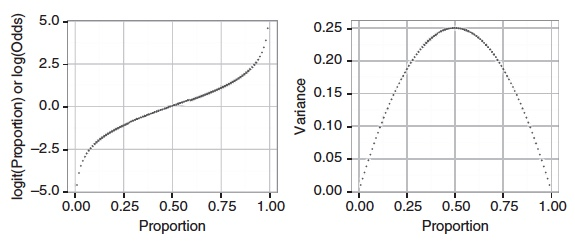
\includegraphics{images/Box9.2.jpeg}

The logistic transformation converts proportions to logits.
\textbf{\emph{Logits are the natural log of the odds and the odds are
the ratio of successes to failures.}} If we had a binomial denominator
of ten with five successes to five failures then the logit would be
log(5/5) = 0.

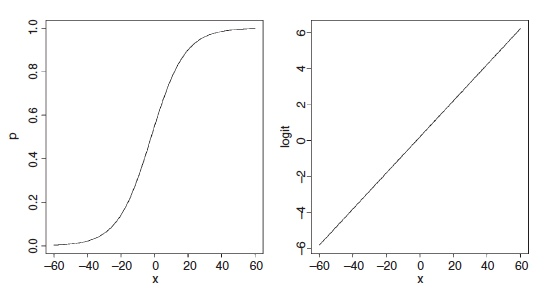
\includegraphics{images/crawley_p_to_logit.jpeg}

So why not simply use the logit transformation and analyse the resulting
logits with a normal least squares regression? Because the variance is
not constant: as we said it is larger at intermediate proportions and
decreases towards both extremes. Instead we use a binomial variance
function to model the variability.

We use the \textbf{family} argument to specify the \textbf{binomial}
distribution (for which the logistic is the default link function). The
logistic link function and binomial distribution take account of the
properties and constraints on the pattern of the mean and variance for
binomial count data.

\begin{Shaded}
\begin{Highlighting}[]
\NormalTok{m1 }\OtherTok{\textless{}{-}} \FunctionTok{glm}\NormalTok{(}\FunctionTok{cbind}\NormalTok{(Number\_killed, Number\_survived) }\SpecialCharTok{\textasciitilde{}}\NormalTok{ Dose, }\AttributeTok{data=}\NormalTok{ beetle, }\AttributeTok{family=}\NormalTok{ binomial)}
\CommentTok{\#wr \textless{}{-} glm(Mortality\_rate\textasciitilde{}Dose, data= beetle, family= binomial, weight= Number\_tested)}
\CommentTok{\#alternative by weighted regression}
\end{Highlighting}
\end{Shaded}

\begin{Shaded}
\begin{Highlighting}[]
\FunctionTok{ggplot}\NormalTok{(beetle,}\FunctionTok{aes}\NormalTok{(Dose,Mortality\_rate)) }\SpecialCharTok{+}\FunctionTok{geom\_point}\NormalTok{() }\SpecialCharTok{+}
  \FunctionTok{geom\_smooth}\NormalTok{(}\AttributeTok{method=}\StringTok{"glm"}\NormalTok{, }\AttributeTok{method.args=}\FunctionTok{list}\NormalTok{(}\AttributeTok{family=}\StringTok{"binomial"}\NormalTok{(}\AttributeTok{link=}\StringTok{"logit"}\NormalTok{)))}\SpecialCharTok{+}
  \FunctionTok{geom\_hline}\NormalTok{(}\AttributeTok{yintercept =} \FunctionTok{mean}\NormalTok{(beetle}\SpecialCharTok{$}\NormalTok{Mortality\_rate), }\AttributeTok{linetype =} \StringTok{"dashed"}\NormalTok{) }\SpecialCharTok{+}
  \FunctionTok{labs}\NormalTok{(}\AttributeTok{title=}\StringTok{"GLM, binomial count (live/die)"}\NormalTok{)}
\end{Highlighting}
\end{Shaded}

\includegraphics{GLM_binary_files/figure-latex/unnamed-chunk-2-1.pdf}

The proportion of beetles killed (Mortality rate) as a function of
increasing concentration of carbon disulphide (Dose).The CI for the
slope does not contain zero, supporting an increasing probability of
mortality as dose increases, as we would expect.

\begin{Shaded}
\begin{Highlighting}[]
\FunctionTok{coef}\NormalTok{(m1)}
\end{Highlighting}
\end{Shaded}

\begin{verbatim}
## (Intercept)        Dose 
##      -14.58        0.25
\end{verbatim}

\begin{Shaded}
\begin{Highlighting}[]
\FunctionTok{confint}\NormalTok{(m1)}
\end{Highlighting}
\end{Shaded}

\begin{verbatim}
## Waiting for profiling to be done...
\end{verbatim}

\begin{verbatim}
##              2.5 % 97.5 %
## (Intercept) -17.26 -12.16
## Dose          0.21   0.29
\end{verbatim}

\textbf{\emph{The logistic curve is linear on the logit scale}} and the
coefficients are the regression intercept (14.6) and slope (0.25) of
this line. The \texttt{summary()} function output gives the same result
in a slightly different form. Lets check the assumption that the ratio
of the residual deviance to the residual DF (which R calls the
\textbf{dispersion parameter}) is approximately 1:1. In this case it is
a little higher (8.43/6=1.4), as we can see from the last line of the
\texttt{summary()} function output:

\begin{Shaded}
\begin{Highlighting}[]
\FunctionTok{summary}\NormalTok{(m1)}
\end{Highlighting}
\end{Shaded}

\begin{verbatim}
## 
## Call:
## glm(formula = cbind(Number_killed, Number_survived) ~ Dose, family = binomial, 
##     data = beetle)
## 
## Deviance Residuals: 
##    Min      1Q  Median      3Q     Max  
## -1.346  -0.452   0.793   1.042   1.326  
## 
## Coefficients:
##             Estimate Std. Error z value Pr(>|z|)    
## (Intercept) -14.5781     1.2985   -11.2   <2e-16 ***
## Dose          0.2455     0.0215    11.4   <2e-16 ***
## ---
## Signif. codes:  0 '***' 0.001 '**' 0.01 '*' 0.05 '.' 0.1 ' ' 1
## 
## (Dispersion parameter for binomial family taken to be 1)
## 
##     Null deviance: 267.6624  on 7  degrees of freedom
## Residual deviance:   8.4379  on 6  degrees of freedom
## AIC: 38.61
## 
## Number of Fisher Scoring iterations: 4
\end{verbatim}

This overdispersion is not too substantial but we can account for it by
using the closely related approach of quasi-maximum likelihood. If we
alter the family to \textbf{quasi-binomial} then instead of being
assumed (and underestimated), the level of variation will be estimated
from the data and the standard errors increased accordingly.

\begin{Shaded}
\begin{Highlighting}[]
\NormalTok{mq1 }\OtherTok{\textless{}{-}} \FunctionTok{glm}\NormalTok{(}\FunctionTok{cbind}\NormalTok{(Number\_survived, Number\_killed) }\SpecialCharTok{\textasciitilde{}}\NormalTok{ Dose, }\AttributeTok{data=}\NormalTok{ beetle, quasibinomial)}
\FunctionTok{summary}\NormalTok{(mq1)}
\end{Highlighting}
\end{Shaded}

\begin{verbatim}
## 
## Call:
## glm(formula = cbind(Number_survived, Number_killed) ~ Dose, family = quasibinomial, 
##     data = beetle)
## 
## Deviance Residuals: 
##    Min      1Q  Median      3Q     Max  
## -1.326  -1.042  -0.793   0.452   1.346  
## 
## Coefficients:
##             Estimate Std. Error t value Pr(>|t|)    
## (Intercept)  14.5781     1.4661    9.94 0.000060 ***
## Dose         -0.2455     0.0243  -10.12 0.000054 ***
## ---
## Signif. codes:  0 '***' 0.001 '**' 0.01 '*' 0.05 '.' 0.1 ' ' 1
## 
## (Dispersion parameter for quasibinomial family taken to be 1.3)
## 
##     Null deviance: 267.6624  on 7  degrees of freedom
## Residual deviance:   8.4379  on 6  degrees of freedom
## AIC: NA
## 
## Number of Fisher Scoring iterations: 4
\end{verbatim}

Notice how the standard errors of the quasibinomial are increased
compared with those from the binomial GLM to take account of the
overdispersion.

However, one disadvantage of quasi-maximum likelihood is that because we
have a quasi-likelihood rather than a true likelihood we are not given a
value for the Akaike information criterion (AIC; although, as we will
see later, some statisticians are willing to calculate quasi-AIC values
and there are R packages that provide them, including the
\texttt{AICcmodavg} package used here).

\textbf{Summary: Binomial Count Data}

\begin{itemize}
\item
  use of the \texttt{glm()} function for analysing binomial count data
  illustrated how we have to bind together the successes and failures
  for the response variable and specify the binomial distribution using
  the \texttt{family} argument.
\item
  We can check whether the level of variability is as assumed by the
  binomial distribution model and inflate the standard errors to account
  for any overdispersion using a quasi-maximum likelihood approach.
\end{itemize}

\textbf{Binary Data}

Binary data are an extreme form of binomial count data in which the
binomial denominator is equal to one, so that every trial produces a
value of either one or zero. Binary data can therefore be analysed using
a GLM with a binomial distribution and the same choice of link functions
to prevent predictions going below zero or above values of one.

However, despite the use of the same distribution and link functions,
because of the constrained nature of the data there are some differences
in the analysis of binomial counts. For one thing, the use of the ratio
of the residual deviance to residual DF to diagnose over- or
underdispersion does not apply. We use \texttt{arm} package
\texttt{binnedplot()} function instead for model checking.

Example: The binary response examining whether or not people switch the
well from which they get their drinking water in relation to the level
of arsenic and the distance to the nearest safe well. 1=safe level of
arsenic, 0=unsafe level.

\begin{Shaded}
\begin{Highlighting}[]
\NormalTok{wells }\OtherTok{\textless{}{-}} \FunctionTok{read.delim}\NormalTok{(}\StringTok{"Binary\_Wells.txt"}\NormalTok{)}
\FunctionTok{ggplot}\NormalTok{(wells,}\FunctionTok{aes}\NormalTok{(dist,}\ControlFlowTok{switch}\NormalTok{)) }\SpecialCharTok{+}\FunctionTok{geom\_point}\NormalTok{() }\SpecialCharTok{+}
  \FunctionTok{geom\_smooth}\NormalTok{() }\SpecialCharTok{+}
  \FunctionTok{xlab}\NormalTok{ (}\StringTok{"Distance to Nearest Well"}\NormalTok{) }\SpecialCharTok{+}
  \FunctionTok{ylab}\NormalTok{ (}\StringTok{"Probability of Switching"}\NormalTok{)}
\end{Highlighting}
\end{Shaded}

\begin{verbatim}
## `geom_smooth()` using method = 'gam' and formula 'y ~ s(x, bs = "cs")'
\end{verbatim}

\includegraphics{GLM_binary_files/figure-latex/Wells: Chart to see raw fit-1.pdf}

It looks like the probability of switching declines with distance, as we
would expect (Fig. 9.2). Before we fit the GLM we can avoid
inconveniently small coefficient values by rescaling distance in
hundreds of meters.

\begin{Shaded}
\begin{Highlighting}[]
\NormalTok{wells}\SpecialCharTok{$}\NormalTok{dist100 }\OtherTok{\textless{}{-}}\NormalTok{ wells}\SpecialCharTok{$}\NormalTok{dist}\SpecialCharTok{/}\DecValTok{100}
\NormalTok{fit}\FloatTok{.1} \OtherTok{\textless{}{-}} \FunctionTok{glm}\NormalTok{(}\ControlFlowTok{switch}\SpecialCharTok{\textasciitilde{}}\NormalTok{dist100, }\AttributeTok{data=}\NormalTok{wells, }\FunctionTok{binomial}\NormalTok{(}\AttributeTok{link=}\StringTok{"logit"}\NormalTok{))}
\FunctionTok{autoplot}\NormalTok{(fit}\FloatTok{.1}\NormalTok{)}
\end{Highlighting}
\end{Shaded}

\begin{verbatim}
## Warning: `arrange_()` was deprecated in dplyr 0.7.0.
## Please use `arrange()` instead.
## See vignette('programming') for more help
\end{verbatim}

\includegraphics{GLM_binary_files/figure-latex/Figure 9.3-1.pdf}

The logistic link function is the default for the binomial variance
function. With a normal least squares analysis we could use the
automatic diagnostic plots to examine the residuals but \textbf{the
constrained nature of binary data makes them of little if any use} (Fig.
9.3).

As already mentioned, we cannot use the ratio of the residual deviance
to residual DF to look for overdispersion as we do with binomial counts
(and Poisson GLMs). Luckily the \texttt{arm} package provides the
\texttt{binnedplot()} function that offers a graphical approach.

\begin{Shaded}
\begin{Highlighting}[]
\FunctionTok{library}\NormalTok{(arm)}
\NormalTok{x }\OtherTok{\textless{}{-}} \FunctionTok{predict}\NormalTok{(fit}\FloatTok{.1}\NormalTok{)}
\NormalTok{y }\OtherTok{\textless{}{-}} \FunctionTok{resid}\NormalTok{(fit}\FloatTok{.1}\NormalTok{)}
\FunctionTok{binnedplot}\NormalTok{(x, y)}
\end{Highlighting}
\end{Shaded}

\includegraphics{GLM_binary_files/figure-latex/Figure 9.4-1.pdf}

The grey lines in the plot indicate ±2 standard errors, within which
approximately 95\% of the binned residuals are expected to fall.

\begin{Shaded}
\begin{Highlighting}[]
\FunctionTok{coef}\NormalTok{(fit}\FloatTok{.1}\NormalTok{)}
\end{Highlighting}
\end{Shaded}

\begin{verbatim}
## (Intercept)     dist100 
##        0.61       -0.62
\end{verbatim}

\begin{Shaded}
\begin{Highlighting}[]
\FunctionTok{confint}\NormalTok{(fit}\FloatTok{.1}\NormalTok{)}
\end{Highlighting}
\end{Shaded}

\begin{verbatim}
## Waiting for profiling to be done...
\end{verbatim}

\begin{verbatim}
##             2.5 % 97.5 %
## (Intercept)  0.49   0.72
## dist100     -0.81  -0.43
\end{verbatim}

It does indeed seem to be the case that the further away an alternative
well is, the less likely people are to switch to it.

Gelman and Hill promote a rough rule of thumb for interpreting the slope
of the logistic regression: the `divide by four rule'. Dividing the
slope coefficient for the logistic regression slope by four will give us
an approximate estimate for the maximum predicted effect on the response
of a unit change in the predictor.

In this case, a difference in distance of 100 m corresponds to a
decrease in the probability of switching of 15\% since --0.62/4 =
--0.15. The figures show the average probability of switching with a
95\% CI.

\begin{Shaded}
\begin{Highlighting}[]
\FunctionTok{ggplot}\NormalTok{(wells, }\FunctionTok{aes}\NormalTok{(dist,}\ControlFlowTok{switch}\NormalTok{)) }\SpecialCharTok{+}
         \FunctionTok{geom\_point}\NormalTok{() }\SpecialCharTok{+}
         \FunctionTok{geom\_smooth}\NormalTok{(}\AttributeTok{method=}\StringTok{"glm"}\NormalTok{, }\AttributeTok{method.args=}\FunctionTok{list}\NormalTok{(}\AttributeTok{family=}\StringTok{"binomial"}\NormalTok{(}\AttributeTok{link=}\StringTok{"logit"}\NormalTok{))) }\SpecialCharTok{+} 
         \FunctionTok{xlab}\NormalTok{ (}\StringTok{"Distance to Nearest Well"}\NormalTok{) }\SpecialCharTok{+}
         \FunctionTok{ylab}\NormalTok{ (}\StringTok{"Probability of Switching"}\NormalTok{)}
\end{Highlighting}
\end{Shaded}

\begin{verbatim}
## `geom_smooth()` using formula 'y ~ x'
\end{verbatim}

\includegraphics{GLM_binary_files/figure-latex/Figure 9.5-1.pdf}

We can look at the effect of arsenic concentration in a similar way:

\begin{Shaded}
\begin{Highlighting}[]
\NormalTok{fit}\FloatTok{.2} \OtherTok{\textless{}{-}} \FunctionTok{glm}\NormalTok{(}\ControlFlowTok{switch}\SpecialCharTok{\textasciitilde{}}\NormalTok{arsenic, }\FunctionTok{binomial}\NormalTok{(}\AttributeTok{link=}\StringTok{"logit"}\NormalTok{), }\AttributeTok{data=}\NormalTok{ wells)}
\FunctionTok{display}\NormalTok{(fit}\FloatTok{.2}\NormalTok{)}
\end{Highlighting}
\end{Shaded}

\begin{verbatim}
## glm(formula = switch ~ arsenic, family = binomial(link = "logit"), 
##     data = wells)
##             coef.est coef.se
## (Intercept) -0.31     0.07  
## arsenic      0.38     0.04  
## ---
##   n = 3020, k = 2
##   residual deviance = 4008.7, null deviance = 4118.1 (difference = 109.4)
\end{verbatim}

Once again, the estimates are in logits with a clear positive effect of
increasing arsenic concentration on the probability of switching wells,
as expected.

\begin{Shaded}
\begin{Highlighting}[]
\FunctionTok{ggplot}\NormalTok{(wells, }\FunctionTok{aes}\NormalTok{(arsenic,}\ControlFlowTok{switch}\NormalTok{)) }\SpecialCharTok{+}
         \FunctionTok{geom\_point}\NormalTok{() }\SpecialCharTok{+}
         \FunctionTok{geom\_smooth}\NormalTok{(}\AttributeTok{method=}\StringTok{"glm"}\NormalTok{, }\AttributeTok{method.args=}\FunctionTok{list}\NormalTok{(}\AttributeTok{family=}\StringTok{"binomial"}\NormalTok{(}\AttributeTok{link=}\StringTok{"logit"}\NormalTok{))) }\SpecialCharTok{+} 
         \FunctionTok{xlab}\NormalTok{ (}\StringTok{"Arsenic Concentration ug/Liter"}\NormalTok{) }\SpecialCharTok{+}
         \FunctionTok{ylab}\NormalTok{ (}\StringTok{"Probability of Switching"}\NormalTok{)}
\end{Highlighting}
\end{Shaded}

\begin{verbatim}
## `geom_smooth()` using formula 'y ~ x'
\end{verbatim}

\includegraphics{GLM_binary_files/figure-latex/Figure 9.6-1.pdf}\\
\strut \\
Lets look at \textbf{Arsenic concentration} AND \textbf{Distance to a
Safe Well} in the same model; this way we can also test for interaction
effects to see if there is a trade off.

Before fitting the GLM we can make life easier by \emph{centering the
explanatory variables by subtracting their mean value}. This has
advantages when a regression intercept of zero is unhelpful or makes no
sense (as with a distance of zero meters here---if we took this
literally the new and old well would be in the same place) and when
examining interactions:

\begin{Shaded}
\begin{Highlighting}[]
\NormalTok{wells}\SpecialCharTok{$}\NormalTok{c.dist100 }\OtherTok{\textless{}{-}}\NormalTok{ wells}\SpecialCharTok{$}\NormalTok{dist100 }\SpecialCharTok{{-}} \FunctionTok{mean}\NormalTok{(wells}\SpecialCharTok{$}\NormalTok{dist100)}
\NormalTok{wells}\SpecialCharTok{$}\NormalTok{c.arsenic }\OtherTok{\textless{}{-}}\NormalTok{ wells}\SpecialCharTok{$}\NormalTok{arsenic }\SpecialCharTok{{-}} \FunctionTok{mean}\NormalTok{(wells}\SpecialCharTok{$}\NormalTok{arsenic)}
\NormalTok{fit}\FloatTok{.5} \OtherTok{\textless{}{-}} \FunctionTok{glm}\NormalTok{(}\ControlFlowTok{switch}\SpecialCharTok{\textasciitilde{}}\NormalTok{c.dist100}\SpecialCharTok{+}\NormalTok{c.arsenic}\SpecialCharTok{+}\NormalTok{c.dist100}\SpecialCharTok{:}\NormalTok{c.arsenic,}
\NormalTok{binomial, }\AttributeTok{data=}\NormalTok{ wells)}
\FunctionTok{display}\NormalTok{(fit}\FloatTok{.5}\NormalTok{) }\CommentTok{\# model numbering from Gelman and Hill}
\end{Highlighting}
\end{Shaded}

\begin{verbatim}
## glm(formula = switch ~ c.dist100 + c.arsenic + c.dist100:c.arsenic, 
##     family = binomial, data = wells)
##                     coef.est coef.se
## (Intercept)          0.35     0.04  
## c.dist100           -0.87     0.10  
## c.arsenic            0.47     0.04  
## c.dist100:c.arsenic -0.18     0.10  
## ---
##   n = 3020, k = 4
##   residual deviance = 3927.6, null deviance = 4118.1 (difference = 190.5)
\end{verbatim}

The coefficients are all given on the \textbf{logit scale}.
{Back-transforming the estimate for the intercept (using the
\texttt{invlogit()} function displayed below) gives the probability of
switching}---because we have centered both variables this is the
probability of switching at average arsenic levels and average distance
to the nearest safe well:

\begin{Shaded}
\begin{Highlighting}[]
\NormalTok{invlogit }\OtherTok{\textless{}{-}} \ControlFlowTok{function}\NormalTok{(x) \{}\DecValTok{1} \SpecialCharTok{/}\NormalTok{ ( }\DecValTok{1}\SpecialCharTok{+}\FunctionTok{exp}\NormalTok{(}\SpecialCharTok{{-}}\NormalTok{x) ) \} }
\FunctionTok{invlogit}\NormalTok{(}\FunctionTok{coef}\NormalTok{(fit}\FloatTok{.5}\NormalTok{)) }\CommentTok{\#for interpreting centered data only?}
\end{Highlighting}
\end{Shaded}

\begin{verbatim}
##         (Intercept)           c.dist100           c.arsenic c.dist100:c.arsenic 
##                0.59                0.29                0.62                0.46
\end{verbatim}

\begin{Shaded}
\begin{Highlighting}[]
\FunctionTok{exp}\NormalTok{(}\FunctionTok{coef}\NormalTok{(fit}\FloatTok{.5}\NormalTok{)) }\CommentTok{\#more books say use exponential; maybe only for poisson}
\end{Highlighting}
\end{Shaded}

\begin{verbatim}
##         (Intercept)           c.dist100           c.arsenic c.dist100:c.arsenic 
##                1.42                0.42                1.60                0.84
\end{verbatim}

The probability of switching at average arsenic levels and average
distance to the nearest safe well is \textbf{0.59}.

\textbf{c.dist100} The effect of a change of 100 m when arsenic is at
average levels is \textbf{-0.87} change in the log-odds (logit).
(proportion = 0.29)

\textbf{c.arsenic} The effect of a unit change (1 ug/L) in arsenic for a
well at average distance is \textbf{0.47} change in the log-odds
(logit). (proportion = 0.62)

\textbf{c.dist100:c.arsenic} For every increase of 100 m we add
\textbf{--0.18} to the log-odds for arsenic. This means that the effect
of the level of arsenic declines with distance to the nearest well.
Similarly, for every unit increase in arsenic we add \textbf{--0.18} to
the log-odds for distance. In other words the higher the arsenic levels
the less important the distance to the nearest safe well. (proportion =
0.46)

So far we have focused on effect sizes (intercepts and slopes), but what
about P-values?

The size of the estimated difference (--0.18) for the interaction is a
bit less than twice the standard error of the difference (0.1), so while
it is marginally significant it fails to meet the conventional 5\% level
(as you can explore using the \texttt{confint()} function CIs, the
\texttt{summary()} function Z-values, or the likelihood ratio test
produced by applying the \texttt{anova()} function to a pair of models
with and without the interaction).

\begin{Shaded}
\begin{Highlighting}[]
\FunctionTok{confint}\NormalTok{(fit}\FloatTok{.5}\NormalTok{)}
\end{Highlighting}
\end{Shaded}

\begin{verbatim}
## Waiting for profiling to be done...
\end{verbatim}

\begin{verbatim}
##                     2.5 % 97.5 %
## (Intercept)          0.27  0.430
## c.dist100           -1.08 -0.670
## c.arsenic            0.39  0.553
## c.dist100:c.arsenic -0.38  0.022
\end{verbatim}

\begin{Shaded}
\begin{Highlighting}[]
\FunctionTok{summary}\NormalTok{(fit}\FloatTok{.5}\NormalTok{)}
\end{Highlighting}
\end{Shaded}

\begin{verbatim}
## 
## Call:
## glm(formula = switch ~ c.dist100 + c.arsenic + c.dist100:c.arsenic, 
##     family = binomial, data = wells)
## 
## Deviance Residuals: 
##    Min      1Q  Median      3Q     Max  
##  -2.78   -1.20    0.77    1.08    1.85  
## 
## Coefficients:
##                     Estimate Std. Error z value Pr(>|z|)    
## (Intercept)           0.3511     0.0399    8.81   <2e-16 ***
## c.dist100            -0.8737     0.1048   -8.34   <2e-16 ***
## c.arsenic             0.4695     0.0421   11.16   <2e-16 ***
## c.dist100:c.arsenic  -0.1789     0.1023   -1.75     0.08 .  
## ---
## Signif. codes:  0 '***' 0.001 '**' 0.01 '*' 0.05 '.' 0.1 ' ' 1
## 
## (Dispersion parameter for binomial family taken to be 1)
## 
##     Null deviance: 4118.1  on 3019  degrees of freedom
## Residual deviance: 3927.6  on 3016  degrees of freedom
## AIC: 3936
## 
## Number of Fisher Scoring iterations: 4
\end{verbatim}

\textbf{Summary: Binary Data}

\begin{itemize}
\item
  We can analyse binary data using a binomial GLM. However, we do not
  use the ratio of the residual deviance to residual DF to diagnose
  over- or underdispersion.
\item
  We can use the \texttt{binnedplot()} function from the arm package to
  examine the binned residuals
\item
  Since the GLM uses the binomial distribution and the logit link
  function, the analysis is interpreted in a similar way to the GLM of
  binomial count data.
\item
  In this case, the GLM of the binary wells data reveals a positive
  effect of arsenic concentration on the probability of switching wells
  and a negative effect of distance to the nearest safe well.
\item
  There is a marginal negative interaction that suggests that each
  effect slightly reduces the effect of the other (the effect of
  distance to the nearest well is a bit reduced as arsenic concentration
  increases and the effect of arsenic concentration is slightly
  moderated as distance to the nearest safe well increases).
\end{itemize}

\textbf{Notes on Interpreting Logistic Coefficients} (Gelman and Hill
2006 and
\url{https://bookdown.org/jefftemplewebb/IS-6489/logistic-regression.html})

The x values, ranging from -6 to 6, are compressed by the inverse logit
function into the 0-1 range. The inverse logit is curved, so the
expected difference in y corresponding to a fixed difference in x is not
constant. At low values and high values of x a unit change corresponds
to very little change in y , whereas in the middle of the curve a small
change in x corresponds to a relatively large change in y . In linear
regression the expected difference in y corresponding to a fixed
difference in x is, by contrast, constant. \textbf{Thus, when we
interpret logistic results we must choose where on the curve we want to
evaluate the probability of the outcome, given the model.}

Coefficients in logistic regression can be challenging to interpret
because of the nonlinearity. There are three approaches that may work:

\begin{enumerate}
\def\labelenumi{\arabic{enumi}.}
\tightlist
\item
  Evaluation at and near the mean of the data (\texttt{invlogit} at
  mean; Gelman and Hill p.81) Works for both categorical and continuous
  linear predictors to \emph{probabilities}.
\end{enumerate}

\texttt{invlogit}(coef(fit.1){[}1{]} +
coef(fit.1){[}2{]}*mean(pred.variable))

\texttt{invlogit}(-1.40 + 0.33*mean(income))

Example; With mean income = 3.1, yielding \emph{Pr(Bush support) = 0.40
at this central point (the mean)}.

\begin{enumerate}
\def\labelenumi{\arabic{enumi}.}
\setcounter{enumi}{1}
\tightlist
\item
  The ``divide by 4 rule''
\end{enumerate}

As a rule of convenience, we can take logistic regression coefficients
(other than the constant term) and divide them by 4 to get an upper
bound of the \emph{predictive difference corresponding to a unit
difference in x}. This upper bound is a reasonable approximation near
the midpoint of the logistic curve, where probabilities are close to
0.5.

For example, in the model Pr(Bush support) = logit\^{}-1(-1.40 + 0.33 ·
income), we can divide 0.33/4 to get 0.08: a difference of 1 in income
category corresponds to no more than an 8\% positive difference in the
\emph{probability} of supporting Bush.

\begin{enumerate}
\def\labelenumi{\arabic{enumi}.}
\setcounter{enumi}{2}
\tightlist
\item
  Interpretation of coefficients as odds ratios
\end{enumerate}

TBD.

\end{document}
